%This is the second chapter of the dissertation

%The following command starts your chapter. If you want different titles used in your ToC and at the top of the page throughout the chapter, you can specify those values here. Since Columbia doesn't want extra information in the headers and footers, the "Top of Page Title" value won't actually appear.

\pagestyle{cu}
\graphicspath{{./Chapter2/Figures/}}
\chapter[Liquid Xenon and Time Projection Chambers][Liquid Xenon and Time Projection Chambers]{Liquid Xenon and Time Projection Chambers}
\label{chap:liquid_xe}

Liquid xenon (LXe) direct detection experiments have led the field for spin-independent WIMP searches with masses $\gtrsim 20$ for roughly
a decade.  More so than liquid argon (LAr), LXe results have been paved the way to new limits, surpassing on the way only those of
other
LXe experiments.

Commercial business, such as steelmaking and coal gasification, rely relatively pure oxygen or nitrogen.  During the separation,
the small amount of xenon and krypton in the air is extracted into a mixture as a by-product.  A distillation process can uncouple
the two, leaving highly pure xenon.

This chapter begins by discussing general properties of xenon and why it is such an effective element for a dark matter search
(\secref{sec:properties}) followed by a summary of signal production (\secref{sec:scintillation}) and then determining the type of
interaction based on its signal properties (\secref{sec:interactions}).

%====================================
\section{General Properties}
\label{sec:properties}
Xenon is a noble gas with atomic number 54 with and a mean molar mass of 131.293 g mol$^{-1}$.  It is the heaviest non-radioactive noble
gas and due to its full valence electron
shell rarely undergoes chemical reactions.  It has a concentration of 87 parts per billion (ppb)
in the Earth's atmosphere at a density of
5.894 g l$^{-1}$.  The phase diagram for xenon is shown in \figref{fig:phase_diagram} and \tabref{tab:xe_properties} lists general
chemical properties.

\begin{figure}
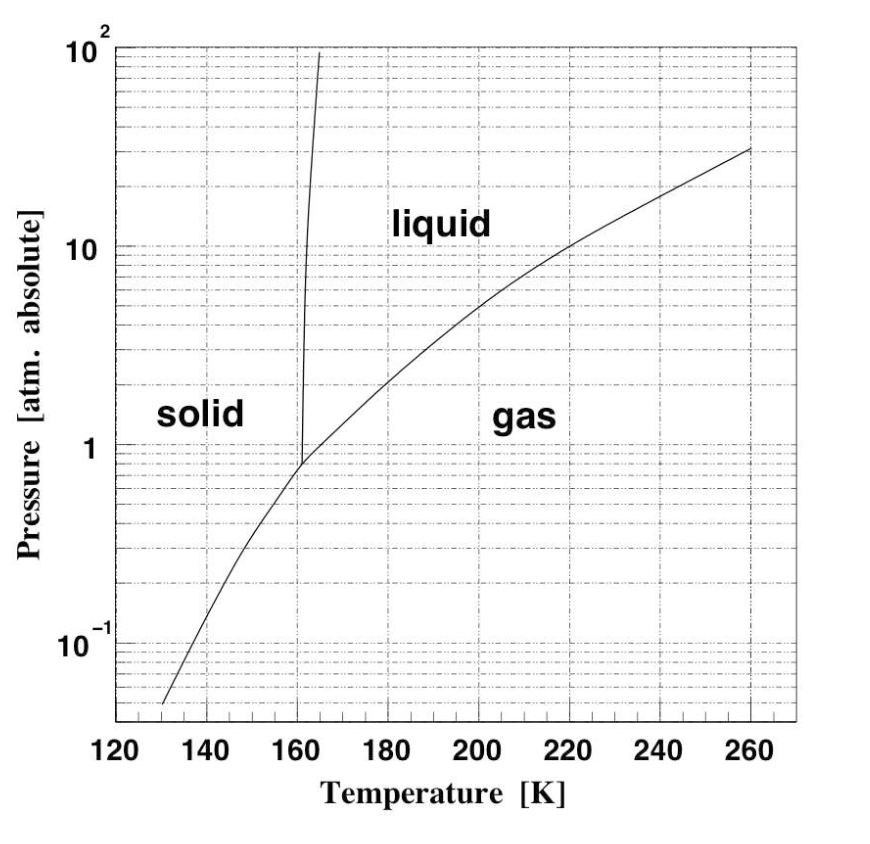
\includegraphics[width=0.6\textwidth]{PhaseDiagram}
\caption{Phase diagram of xenon.  Image credit: \citeref{Aprile2009}.}
\label{fig:phase_diagram}
\end{figure}
 
\begin{table}[t]
 \centering
 \begin{tabular}{cc}
 \hline
 \hline
 Chemical Property & Value \\
 \hline
 Atomic Number & 54 \\
 Molar mass & 131.293 g mol$^{-1}$ \\
 Melting point (1 atm) & 161.4 K \\
 Boiling point (1 atm) & 165.0 K \\
 Density as gas (298 K, 1 atm)  &  5.40 g l$^{-1}$ \\
 Density as gas (165 K, 1 atm)  &  9.99 g l$^{-1}$ \\
 Density as liquid (165 K, 1 atm) & 2.94 g cm$^{-3}$ \\
 Critical point & $16.59^{\circ}$C, 57.65 atm, 1.155 g cm$^{-3}$ \\
 Dielectric constant & 1.95 \\
 Triple point & $-111.74^{\circ}$C, 0.805 atm, 3.08 g cm$^{-3}$ \\
 Thermal conductivity & $5.65 \times 10^{-3}\ \mathrm{W\ m^{-1}\ K^{-1}}$ \\
 Covalent radius & $140 \pm 9$ pm \\
 \hline
 \hline
 \end{tabular}
 \caption{Chemical properties for xenon.  Data taken from \citeref{Baudis2014}.}
\label{tab:xe_properties}
\end{table}

The naturally occurring xenon isotopes are listed in \tabref{tab:xe_isotopes}.  \ce{^{136}Xe}, which makes up 8.8573\% of natural xenon,
has been measured to undergo double beta decay with a half-life of $t_{1/2} > 2.4 \times 10^{21}\ \mathrm{y}$.  \ce{^{124}Xe},
\ce{^{126}Xe},
and \ce{^{134}Xe} are also predicted to to be unstable but decays have not been observed so they are not considered when building a
liquid xenon detector or analyzing data \citeref{Barros2014}.

Unstable isotopes with $t_{1/2} > 1\ \mathrm{h}$ are given in \tabref{tab:xe_unstable_isotopes}.  The longest-lived isotope is
\ce{^{127}Xe} with $t_{1/2} = 36.4\ \mathrm{d}$.  Also listed are metastable states $\mathrm{^{129m}Xe}$, $\mathrm{^{131m}Xe}$, and
$\mathrm{^{133m}Xe}$ with energies 163.9, 236.2, and 233.2 keV $\gamma$-rays, respectively.  $\mathrm{^{129m}Xe}$ and $\mathrm{^{131m}Xe}$
are more commonly produced since \ce{^{129}Xe} and \ce{^{131}Xe} are stable and make up $> 47\%$ of natural xenon
(\tabref{tab:xe_isotopes}).  Following a nuclear recoil calibration they are used to measure a number of properties about our detector
including the electron lifetime (\secref{subsec:electron_lifetimes_measurement_gammas}).  Their shorter-lived 39.6
(\ce{^{129}Xe}) and 80.2 (\ce{^{131}Xe}) keV nuclear
excited states, which have $t_{1/2} = 0.97\ \mathrm{ns}$ and 0.48 ns, respectively, are rarely resolvable from the signal of the
particle-nucleus scatter.

Xenon has several advantages that make it a good target for dark matter detection.  At \$2000/kg it is scaleable for larger
detectors.  Its high molar mass provides excellent self-shielding, which reduces background contamination in the region of interest due to
external radiation
(\secref{subsec:backgrounds_detector_materials}).  Furthermore, nearly 50\% of naturally occurring xenon is $^{129}$Xe or $^{131}$Xe,
which gives it sensitivity to spin-dependent interactions.  Its production of light and charge - referred to as light and charge yields
(\secref{subsubsec:er_nr_calibrations_results_ly_qy}) - are among the highest noble gases.  Finally, the expected background contribution
from xenon itself comes just from \ce{^{136}Xe} so is extremely small (\tabref{tab:xe_isotopes}).  Therefore
intrinsic radioactivity comes almost entirely from trace amounts of other radioactive noble gases, which can be reduced
(\secref{subsec:xenon1t_kr_dist}).


\begin{table}
 \centering
 \begin{tabular}{ccccc}
 \hline
 \hline
 Isotope & Natural Abundance [\%] & Spin & Half-life & Decay mode \\
 \hline
 $^{124}$Xe & 0.0952 & 0 &  $> 1.6 \times 10^{14}\ \mathrm{y}$ & $2\nu \beta^{+} \beta^{+}$ \\
 $^{126}$Xe & 0.089 & 0 & $> 4.7 \mdash 12 \times 10^{25}\ \mathrm{y}$ & $2\nu \beta^{+} \beta^{+}$ \\
 $^{128}$Xe & 1.910 & 0 & stable & $-$ \\
 $^{129}$Xe & 26.401 & 1/2 & stable & $-$ \\
 $^{130}$Xe & 4.071 & 0 & stable & $-$ \\
 $^{131}$Xe & 21.23 & 3/2 & stable & $-$ \\
 $^{132}$Xe & 26.909 & 0 & stable & $-$ \\
 $^{134}$Xe & 10.436 & 0 &  $> 5.8 \times 10^{22}\ \mathrm{y}$ & $2\nu \beta^{-} \beta^{-}$ \\
 $^{136}$Xe & 8.857 & 0 &  $> 2.4 \times 10^{21}\ \mathrm{y}$ & $2\nu \beta^{-} \beta^{-}$ \\
 \hline
 \hline
 \end{tabular}
 \caption{Properties of naturally occurring xenon isotopes.  Decays of \ce{^{124}Xe}, \ce{^{126}Xe}, and \ce{^{134}Xe} have not been
 observed but are predicted.  \ce{^{124}Xe} is predicted to also decay by $2 \nu \beta^+ \mathrm{EC}$ and
 $2 \nu \mathrm{ECEC}$.  Half-life and decay information is taken from \citeref{Singh2007, Barros2014}.}
\label{tab:xe_isotopes}
\end{table}

\begin{table}
\centering
\begin{tabular}{ccccc}
\hline
\hline
Isotope & Spin & Half-life & Decay mode & Decay product \\
\hline
$^{122}$Xe & 0 & 20.1 h & EC & \ce{^{122}I} \\
$^{123}$Xe & 1/2 & 2.08 h & EC & \ce{^{123}I} \\
\ce{^{125}Xe} & 1/2 & 17.1 h & EC & \ce{^{125}I} \\
\ce{^{127}Xe} & 1/2 & 36.4 d & EC & \ce{^{127}I} \\
$\mathrm{^{129m}Xe}$ & 11/2 & 8.88 d & $\gamma$-ray & ground state \\
$\mathrm{^{131m}Xe}$ & 11/2 & 11.93 d & $\gamma$-ray & ground state \\
\ce{^{133}Xe} & 3/2 & 5.24 d & $\beta^-$ & \ce{^{133}Cs} \\
$\mathrm{^{133m}Xe}$ & 11/2 & 2.19 d & $\gamma$-ray & ground state \\
\ce{^{135}Xe} & 3/2 & 9.14 h & $\beta^-$ & \ce{^{135}Cs} \\
\hline
\hline
\end{tabular}
\caption{Unstable isotopes of xenon with half-lifes of $> 1\ \mathrm{hr}$.  Spins, half-lifes, decay modes, and decay products are
listed.}
\label{tab:xe_unstable_isotopes}
\end{table}

\begin{figure}
\centering
\includegraphics[width=0.8\textwidth]{Figure 1 from SeeFig15}
\end{figure}



%====================================
\section{Signal Production}
\label{sec:scintillation}
As radiation scatters off a xenon atom it will cause photon emission due to two effects.  The first is electrons excited to
higher orbitals will quickly de-excite, with the energy carried away by photons.  The second possibility is ionized xenon may
recombine with an
electron (can but doesn't need to be its own), after which it is in an excited state equivalent to the first scenario.  In the
context of this and other experiments the photons are observed as primary (or prompt) scintillation.  Secondary scintillation results from
electrons that do not recombine and is measured only in a time-projection
chamber (TPC).  This chapter only considers interactions in xenon in the presence of an electric field, unless otherwise
specified.



%========
\subsection{Primary Scintillation}
\label{subsec:primary}
When a particle scatters off a xenon atom it can excite or ionize its valence electrons.  A freed electron can escape or recombine with a
Xe$^{+}$.  Excitons Xe$^{*}$ can bond with another Xe atom to create
dimers, Xe$_{2}^{*}$, commonly referred to as excimers.  The processes of recombination is shown in \eqnref{eq:recomb}, where $Q$
represents heat.

If the interaction occurs in an electric field some $e^{-}$ will be pulled from the site, which lowers recombination and therefore
decreases primary
scintillation and increases secondary scintillation (\secref{subsec:secondary}).  The extent to which recombination changes depends on the
strength of the electric
field.  However, even without a field there will not be
100\% recombination because some of the freed $e^{-}$ will escape the electromagnetic pull of their parent ions.

\begin{subequations}
\begin{align}
\mathrm{Xe}^{+} + \mathrm{Xe} &\rightarrow \mathrm{Xe}_{2}^{+} \\
\mathrm{Xe}_{2}^{+} + e^{-} &\rightarrow \mathrm{Xe}^{**} + \mathrm{Xe} \\
\mathrm{Xe}^{**} &\rightarrow \mathrm{Xe}^{*} + Q
\end{align}
\label{eq:recomb}
\end{subequations}

The Xe$^{*}$ that has results from recombination is equivalent to if it had only ever been excited.  At this point
it de-excites via \eqnref{eq:deexcite}.  Xe$_{2}^{*}$ is in either a singlet
($^{1}\Sigma$) or triplet ($^{3}\Sigma$) state and quickly de-excites to the ground state.

\begin{subequations}
\begin{align}
\mathrm{Xe}^{*} + \mathrm{Xe} &\rightarrow \mathrm{Xe}_{2}^{*} \\
\mathrm{Xe}_{2}^{*} &\rightarrow 2\mathrm{Xe} + \gamma
\label{eq:deexcite_gamma}
\end{align}
\label{eq:deexcite}
\end{subequations}

The average \gammaray in \eqnref{eq:deexcite_gamma} has a wavelength of 178 nm.  Not surprisingly, the number of photons is
anti-correlated with the number of electrons, since for each \electron that
recombines with xenon a \gammaray is emitted.  The lifetimes for the singlet and triplet
excimers are $3.1 \pm 0.7$ ns and $24 \pm 1$ ns, respectively \citeref{Mock2014}.  The singlet-to-triplet ratios for
a number of different interactions are shown in \tabref{tab:singlet_to_triplet}.  Detecting WIMPS requires differentiating between
scatters with the xenon electron shells (electronic recoils) and nucleus (nuclear recoils).  \tabref{tab:singlet_to_triplet} shows that
nuclear recoils result in a higher fraction of singlet states.  Unfortunately the $^1\Sigma$ and $^3\Sigma$ lifetimes
are too short to resolve so they cannot be used for discrimination.  This makes single-phase LXe detectors
less desirable than liquid argon (LAr), which has single and triplet states of $< 6.2$ ns and $1.30 \pm 0.06\ \mathrm{\mu s}$
\citeref{Heindl2011}.

\begin{table}[t]
 \centering
 \begin{tabular}{cc}
 \hline
 \hline
 Event & $^1\Sigma / ^3\Sigma$ \\
 \hline
 ER (direct excitation from $\gamma$) & $0.17 \pm 0.05$ \\
 ER (recombination from $\gamma$) & $0.8 \pm 0.2$ \\
 ER (from $\alpha$) & $2.3 \pm 0.51$ \\
 NR (from neutron) & $7.8 \pm 1.5$ \\
 \hline
 \hline
 \end{tabular}
 \caption{Error-weighted average of world data for single-to-triplet ratios for various scattering cases \citeref{Mock2014}.}
\label{tab:singlet_to_triplet}
\end{table}

\figref{fig:interaction_channels} shows the interaction
channels of $\beta$- or $\gamma$-induced xenon recoils described in \eqnref{eq:recomb} and \eqnref{eq:deexcite}.
However, in nuclear recoils
it has been observed that two excitons may collide and free an electron as shown in \eqnref{eq:biexcitonic} in what is known as
biexcitonic quenching (\secref{subsec:recombination}).

\begin{figure}
\centering
\includegraphics[width=0.8\textwidth]{interaction_channels}
\caption{Signal generation pathways for electronic and nuclear recoils.  Describe paths of electrons.  Image credit: \citeref{Faham2014}.}
\label{fig:interaction_channels}
\end{figure}




%========
\subsection{Secondary Scintillation}
\label{subsec:secondary}
In an electric field $E$ an \electron that is freed but does not recombine with its parent or other ions will move anti-parallel
to the field at drift velocity $v_{d}$.  At fields of $\lesssim 100\ \mathrm{V\ cm^{-1}}$ the drift velocity is nearly proportional to
$E$ and is given by $v_{d} = \mu E$
where $\mu$ is the electron mobility, estimated to be ${\sim}2200\ \mathrm{cm^{2}\ V^{-2}\ s^{-1}}$ at these fields
\citeref{Miller1968}.  As
$E$ increases $v_{d} \propto E^{1/2}$ until approximately $10^4\ \mathrm{V\ cm^{-1}}$ where it flattens at
${\sim} 3\ \mathrm{mm\ \mu s}$.  \figref{fig:drift_velocity} shows \vd
as a function of $E$ and \tabref{tab:drift_velocity} gives the approximate relationship.

In liquid noble gas detectors used for dark matter searches electrons are drifted to the surface of the liquid and
extracted across ${\sim}5\ \mathrm{mm}$ of xenon gas.  As the electrons drift across the gas they excite and ionize new xenon atoms,
creating a second signal referred to as secondary scintillation.  Because the amount of scintillation
produced per electron is independent of the number of electrons extracted this is also known as proportional scintillation.  By
measuring this scintillation the number of \electron extracted can be determined.  Details of \electron drift and proportional
scintillation is found in \secref{subsec:tpcs_working_principle}.

\begin{table}
 \centering
 \begin{tabular}{cc}
 \hline
 \hline
 $E$ [V cm$^{-1}$] & $E$ dependence \\
 \hline
 $\lesssim 100$ & $E$ \\
 ${\sim} 100 \mdash 10^{3 \mdash 4}$ & $E^{1/2}$ \\
 $\gtrsim 10^{4}$ & $-$ \\
 \hline
 \hline
 \caption{Drift velocity \vd as a function of electric field $E$ for LXe}
 \end{tabular}
 \label{tab:drift_velocity}
\end{table}

\begin{figure}
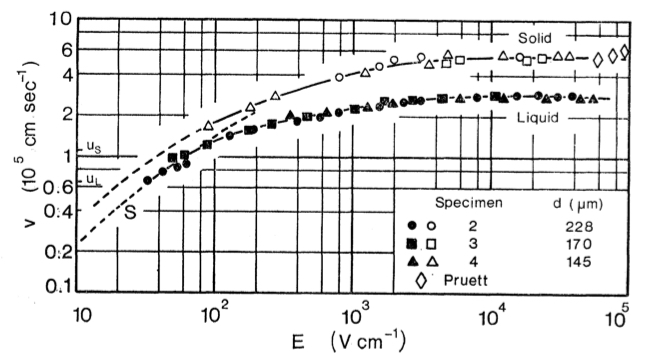
\includegraphics[angle=0.5, width=0.8\textwidth]{DriftVelocity}
\caption{Field-dependent drift velocity for solid ($-116^{\circ}\mathrm{C}$) and liquid ($-110^{\circ}\mathrm{C}$) xenon.  Image credit:
\citeref{Miller1968}.}
\label{fig:drift_velocity}
\end{figure}




%====================================
\subsection{Stopping Power}
\label{subsec:stopping_power}
A particle that loses energy through inelastic collisions with electrons (prompting excitation and ionization) produces an electronic
recoil.  The energy lost per unit
length is the electronic stopping power $S_{\mathrm{elec}}(E) = -(dE/dx)_{\mathrm{elec}}$ ($S_{\mathrm{elec}}$ is positive).  It is
correlated with the linear energy transfer (LET) and depends on the type and energy of the particle and properties of the
medium (e.g. density and composition).  A larger electronic stopping power indicates the particle will slow more quickly and
transfer its energy more densely along its track.  This affects recombination between \electron and ions and is discussed in
\secref{subsec:recombination}.

\begin{figure}[t]
\includegraphics[width=0.8\textwidth]{stopping_power_components}
\caption{Mass stopping power for alphas (blue), $e^{-}$ (green), and protons (pink).  Electronic (long dashed), nuclear (short dashed),
and total (solid) stopping powers for each are shown.  The electronic stopping power is more significant except for $e^-$ at
$\gtrsim 15\ \mathrm{MeV}$.  Data from \citeref{Berger2018a}.}
\label{fig:mass_stopping_power}
\end{figure}

The energy loss per unit length of a particle through elastic collisions with atoms is the nuclear stopping power
$S_{\mathrm{nucl}}(E) = -(dE/dx)_{\mathrm{nucl}}$.  In contrast to electronic stopping power,
$S_{\mathrm{nucl}}(E)$ quantifies the slowing of the particle due to interactions with nuclei of the target and can be calculated using
the repulsive potential energy between atoms.

Dividing the stopping power by the medium's density ($S(E) / \rho$) gives a function of the incident particle known as
the mass stopping power.  Electronic (long dashed) and nuclear (short) mass stopping powers are shown for alphas, electrons, and protons
in \figref{fig:mass_stopping_power}.  $S_{\mathrm{elec}} > S_{\mathrm{nucl}}$ over all energy except for electrons above roughly 15
MeV.  The total stopping power is

\begin{equation}
\bigg( \frac{dE}{dx} \bigg)_{\mathrm{tot}} = \bigg( \frac{dE}{dx} \bigg)_{\mathrm{elec}} + \bigg( \frac{dE}{dx} \bigg)_{\mathrm{nucl}}
\end{equation}

\noindent and is shown as the solid lines in \figref{fig:mass_stopping_power}.  The mean path length of a particle with initial energy
$E_0$ can be approximated by

\begin{equation}
\Delta x = \int_0^{E_0} \frac{1}{S(E)}\, dE
\label{eq:stopping_power_dist_trav}
\end{equation}

\noindent where $\Delta x$ is the continuous slowing down approximation (CSDA) and
$S(E) \equiv -(dE/dx)_{\mathrm{tot}}$.  \eqnref{eq:stopping_power_dist_trav} does not account for energy-loss
fluctuations.  For spin-independent
WIMP dark matter searches the relevant energy range for electrons is $1 \mdash 20$ keV.  In this region $S(E)/\rho$ decreases so
electrons with more energy will travel farther by a ratio greater than their energy.  Alphas do not affect
our dark matter search since they are in the MeV range and are easily identified by their large primary scintillation.  The
\alphadecays that are relevant in our detector sit mostly around 5-7 MeV so have a stopping power between
$200 \mdash 400\ \mathrm{MeV\ cm^2\ g^{-1}}$.  In this region their mass stopping power also decreases with energy.  The $\alpha$ and
proton curves have similar shapes because they are both described by the Bethe formula \citeref{Bethe1937}.

One of the biggest advantages of liquid xenon is its large stopping power (largely due to its high atomic
mass), which provides self-shielding.  Because distance and stopping power are anti-correlated, particles in LXe travel relatively short
distances before stopping.  Self-shielding protects the interior of the detector from outside radiation,
which rarely penetrates more than a few cm
into the LXe, allowing a larger fiducial volume (FV) for dark matter searches.  Because the stopping power is proportional to the
density of the medium, LXe is more effective at self-shielding than liquid argon ($\rho = 1.395\ \mathrm{g\ cm^{-3}}$) and liquid neon
($1.207\ \mathrm{g\ cm^{-3}}$).

\begin{figure}
\centering
\includegraphics[width=\textwidth]{recoil_diagram}
\caption{Electronic (top, $\gamma$) and nuclear (bottom, neutron) recoil tracks for 20 keV scatters.  Excitons (red circles), ions
(blue), and
heat (grey) are marked along the track.  The electronic recoil produces ${\sim} 20 \times$ as many ions as excitons while for nuclear
recoil they are roughly equal.  Heat is only relevant in NRs and leads to signal quenching.  The electronic recoil has a path of
${\sim} 1\ \mathrm{\mu m}$ while the much denser 10 nm of the NR compels higher recombination.  Image credit: \citeref{Faham2014}.}
\label{fig:er_nr_recoil_diagram}
\end{figure}

The track structure from a recoiling electron or xenon nucleus is characterized by the distribution of \electron, ions, excitons, and heat
when all electrons have slowed to sub-excitation speeds \citeref{Chepel2013}.  Tracks are typically cylindrical with secondary branches
from $\delta$-ray.  However, aside from this basic structure they can vary considerably with particle, energy, and
stopping power, and they play a major role in recombination.  \figref{fig:er_nr_recoil_diagram} shows tracks for 20 keV electronic and
nuclear
recoils.  For the electronic recoil a \gammaray ionizes the atom and transfers its energy to the freed electron.  As the electron moves
through the xenon it excites and ionizes more atoms, creating secondary branches from $\delta$-rays until it comes to a rest after
roughly $0.5\ \mathrm{\mu m}$.  The number of ions is ${\sim}20$ times as high as the number of excitons.  Because the \electron only
interacts with the electron shells of the atom not energy is lost as heat.

For the nuclear recoil a 20 keV neutron scatters with a xenon nucleus.  Unlike the electronic recoil where the energy of the \gammaray is
passed to the electron (after small loss from ionization) for a nuclear recoil it is passed to the atom.  The higher stopping power
creates a denser track and a shorter average path length of approximately 10 nm.  In addition to exciting and ionizing, the recoiling atom
passes translational energy to other atoms that cannot be observed (\secref{subsec:recombination}).  The exciton-to-ion ratio is roughly
1, and the higher density of ions leads to greater recombination between electrons and non-parent \ce{Xe^+}.


%========
\subsection{Recombination}
\label{subsec:recombination}
A fraction of atoms that are ionized recombine with electrons.  The recombination fraction depends on a number of parameters
including ionization density
(stopping power, \secref{subsec:stopping_power}), thermal energy of ionized atoms and $e^{-}$, electron mobility, diffusion rate, electric
field, and probability of recombination when an electron and ion meet.

An early theory by Onsager modeled recombination by defining what is now known as the Onsager radius as the distance between an
electron-\ce{Xe^+} pair where the Coulomb energy equals the \electron thermal energy \citeref{Onsager1938}.  An electron within the
Onsager radius will be unable to escape so will recombine with the ion.  At the Onsager radius the probability of escape is $e^{-1}$.  An
\electron
with $E_{\mathrm{thermal}} > E_{\mathrm{Coulomb}}$ should not be influenced by the ion, regardless of the presence of an electric
field.  The thermalization range for LXe is $4000 \mdash 5000$ nm \citeref{Mozumder1995}, far higher than the Onsager radius for liquid
xenon of $49$ nm.  Without an electric field a large fraction of these electrons will recombine on
timescales of $> 1\ \mathrm{ms}$, which because of the short observation window will appear as a decrease in photons, and the electrons
will be classified as having escaped (with an electric field the electrons outside the Onsager radius will drift from the interaction site
and not recombine) \citeref{Doke2002}.

A shortcoming of the Onsager radius is that it treats the interactions between Xe$^{+}$ and \electron as strictly Coulomb.  However,
the high coefficient of polarization of LXe produces dipole moments in the ions, causing the electric field to fall faster than
$1/r$.  In fact, the potential is steep enough that the ion travels via phonon-assisted tunneling \citeref{Thomas1987}, making its
mobility significantly smaller (3-5 orders of magnitude \citeref{Miller1968, Yoshino1976}) than that of the electrons.

As a result of these disparities another model was proposed that includes diffusion but the rate of
recombination depends on
the density of \electron and ions independently \citeref{Jaffe1913}.  Its derivation comes by

\begin{subequations}
\begin{align}
\frac{\partial N_{+}}{\partial t} &= -u_{+} \mathbf{E}_d \cdot \nabla N_{+} + d_{+} \nabla^{2} N_{+} - \alpha N_{+} N_{-}
\label{eq:diff_plus} \\
\frac{\partial N_{-}}{\partial t} &= u_{-} \mathbf{E}_d \cdot \nabla N_{-} + d_{-} \nabla^{2} N_{-} - \alpha N_{+} N_{-}
\label{eq:diff_minus}
\end{align}
\label{eq:diff_plus_mins}
\end{subequations}

\noindent where $N_{\pm}$ are the ion ($+$) and electron ($-$) charge distributions ($N_+ = N_-$), $\mu_{\pm}$ are their mobilities,
$d_{\pm}$ and $\alpha$
are the coefficients for diffusion and recombination, and $\mathbf{E}_d$ is the electric field.  The terms on the right sides of
\eqnref{eq:diff_plus} and \eqnref{eq:diff_minus} correspond to the drift, diffusion, and recombination, from left to right.  The
diffusion in xenon is small (millimeters per drift meter \citeref{Deiters1981}) and can be ignored.  Likewise the ion mobility $\mu_{+}$
is several orders of magnitude smaller than that
of the electron and is disregarded.  Thus \eqnref{eq:diff_plus_mins} can be simplified to

\begin{subequations}
\begin{align}
\frac{\partial N_{+}}{\partial t} &= - \alpha N_{+} N_{-}
\label{eq:diff_simple_plus} \\
\frac{\partial N_{-}}{\partial t} &= u_{-} E_d \frac{\partial N_{-}}{\partial z} - \alpha N_{+} N_{-}
\label{eq:diff_simple_minus}
\end{align}
\end{subequations}

\noindent which, if each electron-ion pair is sufficiently far from all others, can be solved exactly.  After some integration and algebra
(detailed in \citeref{Thomas1987}), the recombination fraction is

\begin{equation}
r = 1 - \frac{\mathrm{ln} (1 + N_0 \varsigma)}{N_0 \varsigma},\ \varsigma = \frac{\alpha}{4 a^{2} u_{-} E_d}
\label{eq:ti_recomb}
\end{equation}

\noindent where $N_0$ is the number of ions and electrons at $t = 0$ that uniformly occupies over a box of dimension $a$.  This is known
as the Thomas-Imel box model \citeref{Thomas1987},
and is successful at explaining recombination measurements including those shown in \figref{fig:ti_recomb}.  Zero recombination
corresponds to
$\varsigma \rightarrow 0$ and complete recombination occurs when $\varsigma \rightarrow \infty$.  In this model $E = 0$ equates to total
recombination, though as mentioned above, this likely occurs outside of the typical observation window.

\begin{figure}
\includegraphics[width=0.8\textwidth]{ti_recombination}
\caption{Measurements of charge collected ($q \propto 1 - r$) for LAr and LXe with respect to $E_d$.  Squares correspond to LXe and were
measured with $\varsigma N_0 E = 0.15\ \mathrm{kV\ cm^{-1}}$.  Triangles and circles are LAr and were measured at
$\varsigma N_0 E = 0.84\ \mathrm{kV\ cm^{-1}}$.  Curves are fits to data using the Thomas-Imdel box model \citeref{Thomas1987}.}
\label{fig:ti_recomb}
\end{figure}

The Thomas-Imel box model works well for short particle tracks but has shortcomings for longer.  At long particle tracks a Birks'
Law (originally developed for organic scintillators, \citeref{Birks1951, Birks1964}) derivation for liquid noble gases yields

\begin{equation}
\frac{dN_{\pm}}{dt} = -\alpha N_{+} N_{-}
\label{eq:birks_diff}
\end{equation}

\noindent for volume recombination - that is, for electrons to recombine with a \ce{Xe^+} that is not their parent.  Here $N_{\pm}$ and
$\alpha$ have the same definitions as in the Thomas-Imel model.  \eqnref{eq:birks_diff} is simplified by assuming
$N_{+} = N_{-}$ and the number of each is proportional to the stopping power $N_{\pm} \propto dE/dx$
(\secref{subsec:stopping_power}).  The latter is only valid for
cylindrical, or long tracks.  Short tracks, which correspond to lower LET and therefore $dE/dx$, are described better by a spherical
excitation-ionization density \citeref{Chepel2013}.  This gives a recombination of

\begin{equation}
r = \frac{A \frac{dE}{dx}}{1 + B \frac{dE}{dx}} + C
\label{eq:birks_recomb}
\end{equation}

\noindent where $A$, $B$, and $C$ are constants derived in the fit \citeref{Doke1988}.  The two terms on the right side of the equation
correspond to
non-geminate and geminate recombination, respectively.  Geminate recombination ($C$) quantifies the
\electron that recombine with their parent ions and is governed by Onsager's model with fixed probability for all $dE/dx$
\citeref{NEST2011}.  Non-geminate
(volume) recombination is when an \electron is captured by an ion different than its parent.  This has been shown to be valid at
$E \gtrsim 80\ \mathrm{keV}$ for \gammarays and light ions, and ${\sim} 1\ \mathrm{MeV}$ electrons.

The considerable LET for $\alpha$-particles creates high-density tracks that lead to strong and quick recombination.  The
density is so high only a small percent of \electron avoid recombination, even at electric fields of
${\sim} 10\ \mathrm{kV\ cm^{-1}}$
(for electrons this is nearly 100\%) \citeref{Chepel2013}.  The consistency in charge collection across different fields causes
difficulties in distinguishing recombination from excitation.

Birk's saturation law explains biexcitonic quenching and the Penning process, which play major roles in nuclear recoils.  Biexcitonic
quenching occurs as

\begin{equation}
\mathrm{Xe}^{*} + \mathrm{Xe}^{*} \rightarrow \mathrm{Xe} + \mathrm{Xe}^{+} + e^{-}
\label{eq:biexcitonic_again}
\end{equation}

\noindent where the \electron escapes with kinetic energy $E = 2E_{\mathrm{ex}} - E_{\mathrm{g}}$ where $E_{\mathrm{ex}}$ and
$E_{\mathrm{g}}$ are the energies of an exciton and band gap, respectively.  The \electron will quickly lose its energy and recombine,
resulting in the emission of a single photon instead of two from the initial excitons.  A second quenching comes from collisions between
excimers via the Penning process that results in an excited and ground molecular states \citeref{Mei2008}.  For nuclear recoils these
quenching factors can be parameterized by

\begin{equation}
f_{b} = \frac{1}{1 + k_B B \frac{dE}{dx}}
\label{eq:nr_scint_quench}
\end{equation}

\noindent where $k_B$ is Birks' constant \citeref{Birks1951, Birks1964}.

The decrease in scintillation yield for $\beta$ and $\gamma$ is only observed at low LET where the ionization density is relatively
low.  The
lack of neighboring $\mathrm{Xe}^{+}$ reduces the probability of recombination with a non-parent ion.  At higher LET the ion density
is sufficient for nearly 100\% recombination and results in the flat region in \figref{fig:scintillation_yield}.  However, unlike nuclear
recoils this there is no true decrease in photons and electrons so this effect does not result in quenching.

\begin{figure}
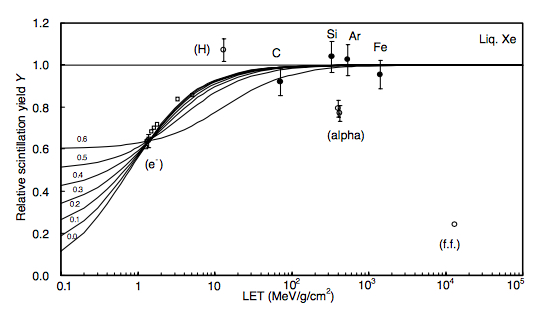
\includegraphics[width=0.8\textwidth]{ScintillationYield}
\caption{Scintillation yield as a function of LET in LXe.  Open circles represent electrons, alpha particles, and fission
fragments.  Solid circles represent relativistic heavy particles.  Open squares mark gamma-rays.  Solid lines trace various fits
to $\beta$-$\gamma$ data from \citeref{Doke2002}.  Image credit: \citeref{Doke2002}.}
\label{fig:scintillation_yield}
\end{figure}



%====================================
\section{Interactions}
\label{sec:interactions}
Because WIMPs are expected to scatter with nuclei electronic recoils are excluded in early analyses (\citeref{Aprile2017f},
\chapref{chap:xenon1t}) as possible signals and considered only as background.\footnote{Results from a WIMP-electron coupling analysis can
be found in \citeref{Aprile2015a}.}  However, understanding the electronic recoil background is necessary to be able to discriminate
against nuclear recoils.  Detector materials have radioactive elements that decay inside the detector, and there are intrinsic
backgrounds such as \krypton and \radon.  The latter is much more concerning since events from
detectors materials cannot breach the inner volume, but intrinsic sources are uniformly distributed throughout the xenon.

To understand our detector calibrations are regularly performed (\secref{subsec:det_char}).  In the ton-scale era of liquid xenon
detectors external sources, which were effective in past experiments, are less efficient because xenon's self-shielding makes it extremely
difficult for radiation to penetrate the interior.  Therefore radioactive
sources that have short half-lifes and can be mixed with the xenon such as $\mathrm{^{83m}Kr}$ and \radoncal are used.  Because these
sources and their progenies have short half-lifes or are stable, they do not contribute to our background after 2-3 days.

\subsection{Photons}
\label{subsec:photons}
Photons produce electronic recoils as they interact with \electron via Compton scattering, pair production, or photoelectric absorption
as shown in \figref{fig:phot_atten}.  Coherent (Rayleigh and Thomson) scattering are also shown though their net energy deposition in the
xenon is zero.

In Compton scattering the photon recoils off of an $e^{-}$ and transfers to it a portion of its energy.  The final energy of the photon
depends only on its initial energy and the scattering angle.  Nuclear Compton scattering is possible but much rarer
\citeref{Christillin1986}.  The low-energy limit of Compton Scattering (photon wavelength larger than particle Compton wavelength) is
Thomson scattering.  Thomson and Rayleigh scattering are elastic so they have a net energy contribution of zero, and are known as coherent
scatters.

Pair production occurs when a high-energy photon produces a particle-antiparticle pair.  Typically this refers to a photon passing
sufficiently
close to an atom's nucleus and creating an electron-positron pair.  The proximity of the nucleus is required to conserve momentum so it
will recoil slightly.  The photon must have an energy of at least twice the electron mass $m_{e}$, or $1.0222\ \mathrm{MeV/c^2}$.  Pair
production
also occurs for a photon in the presence of an atomic electron but is less probable and requires an energy of at least $4m_{e}$.  This
is known as triplet production since the recoiling electron creates a track in addition to the electron-positron pair
\citeref{Hubbell2006}.  At high energies pair production becomes the dominant interaction for photons and matter.

Photoelectric absorption is when an electron absorbs the energy of the photon and is liberated from its electron shell.  In this case the
photon disappears entirely and the kinetic energy of the electron is equal to the photon's energy minus the electron binding
energy.  Photoelectric absorption was helpful for calibrating small detectors using mono-energetic \gammarays from elements such as
\cesium (661.7 keV) and \cobaltsixty
(1.1732 and 1.3325 MeV).  For large detectors self-shielding prevents even high-energy \gammarays from reaching the fiducial
volume, so external sources cannot be used for calibration.  Photoelectric absorption is the dominant interaction in the WIMP search
energy region of interest ($E < 20\ \mathrm{keV}$), and is shown as the red dotted line in \figref{fig:phot_atten}.

\begin{figure}
 \centering
 \includegraphics[width=0.8\textwidth]{photon_scatter}
 \caption{Mass attenuation coefficient and attenuation length for $1\ \mathrm{keV}$ to $100\ \mathrm{MeV}$ photons.  Photoelectric
 absorption (red dashed), Compton scattering (green), coherent (Rayleigh and Thomson) scattering (purple), and pair production (blue) are
 shown in addition to the total (solid black).  The discontinuity at ${\sim}5\ \mathrm{keV}$ occurs just above the binding energy of the
 L-shell electrons and is due to an increase in photoelectric absorption.  A similar process occurs for the K-shell at
 roughly 40 keV.  Data from \citeref{Berger2018b}.}
 \label{fig:phot_atten}
\end{figure}


\subsection[$\beta$-Decays][$\beta$-Decays]{$\mathbf{\beta}$-Decays}
\label{subsec:beta}
\betadecays are the emission of an electron-antineutrino (positron-neutrino) from a neutron (proton).  As with photons, they interact
with the \electron shell and produce electronic recoils.  Because the neutrino carries
some momentum, the energy spectrum of the \electron is not mono-energetic, so it can be difficult to identify the origin of the event.  In
xenon
experiments low-energy \betadecays contribute the most contamination in the search region and occur throughout the entire volume due to
\ce{^{85}Kr} and \ce{^{222}Rn} being uniformly throughout the detector.  \krypton decays via

\begin{equation}
\ce{^{85}Kr} \rightarrow \ce{^{85}Rb} + e^{-} + \overline{\nu_{e}}
\end{equation}

\noindent with an end-point energy of 687 keV and branching ratio of 99.53\% and (remaining 0.47\% is 173 keV plus 514 keV
$\gamma$-rays).  These low-energy \betadecays
contaminate the search region, and their half-life of 10.72 years ensures their presence throughout the lifetime of the experiment.

\ce{^{222}Rn} presents a similar problem.  It is a daughter of the \ce{^{238}U} decay chain emanates from the detector materials.  Like
\ce{^{85}Kr} it is a noble gas so it mixes with the xenon.  Its two most dangerous daughters are \leadtwofourteen and \ce{^{214}Bi}, each
of which
undergo $\beta$-decay.  \ce{^{214}Bi} is easily identifiable because its daughter \poloniumtwofourteen has a half-life of
$160\ \mathrm{\mu s}$ and undergoes $\alpha$-decay.  Thus a cut on coincidence can remove these events.  \leadtwofourteen is more
dangerous because there is no observable hallmark of its decay.  Its end-point energy when it decays to the ground state of
\bismuthtwofourteen

\begin{equation}
\ce{^{214}Pb} \rightarrow \ce{^{214}Bi} + e^{-} + \overline{\nu_{e}}
\end{equation}

\noindent is 1019 keV.  More concerning is a decay to higher energy levels, which
if near the border of the fiducial volume has a risk of the subsequent \gammaray exiting undetected.  In XENON100 recoiling daughters of
the \ce{^{222}Rn} decay chain were observed to drift towards the cathode - possible the result of becoming ionized from parent decays
\citeref{Weber2013} - lowering the number of \betadecays in the region of interest.


\subsection{Neutrinos}
\label{subsec:neutrinos}
Neutrinos impact both electronic and nuclear recoil spectra at low energies.  Solar neutrinos can elastically scatter off \electron
and produce an electronic recoil.  \textit{pp} neutrinos make up 92\% of these scatters, with \ce{^{7}Be} making 7\%, and all other
sources contributing $<1$\% \citeref{Aprile2016a}.

Coherent neutrino-nucleus scattering produces nuclear recoils.  The majority of these interactions in the energy region of interest come
from Solar \ce{^{8}Be}
and \textit{hep} neutrinos, as those at higher energy sources such as diffuse supernovae and Earth's atmosphere have a significantly
lower rate.

Neutrinos are an irreducible background that affects our detector uniformly.  Its contribution scales proportionally with mass so as
detectors continue to grow its contribution will become larger.  The neutrino coherent scattering cross section is shown in
\figref{fig:si_limits}.


\subsection{Neutrons}
\label{subsec:neutrons}
Neutrons in our detector come from two main sources: spontaneous fission (mainly $\alpha$) of elements in primordial chains
\uranium, \ce{^{235}U}, and \ce{^{232}Th} that are present in detector materials (known as radiogenic neutrons), and muons
passing through the rock and material above and around the detector (cosmogenic neutrons).  Radiogenic neutrons have energies in the MeV
range
while cosmogenic can reach tens of GeV \citeref{Aprile2016a}.  Neutrons have a mean free path on the order of ten cm, which makes
them more difficult to shield than $\alpha$, $\beta$, or $\gamma$.  Furthermore, neutrons produce nuclear recoils, which can make
them indistinguishable from WIMPs.  It is critical then to have a thorough understanding of the neutron background so a reliable
calculation of the number of background events in the signal region can be made.  Failing to do so risks mistaking a neutron as a WIMP or
vice versa.

Neutrons will scatter elastically, inelastically, or be radiatively absorbed by xenon nuclei.  Radiative absorption is when the
nucleus captures the neutron, extending its atomic mass by one.  Fortunately, because the number of stable isotopes is large the increase
often leads to another stable
atom.  Exceptions are \ce{^{125}Xe}, \ce{^{127}Xe}, \ce{^{133}Xe}, and \ce{^{135}Xe}, which are listed in \tabref{tab:ncaption_xe}
along with their decays and half-lifes.  \ce{^{125}I} and \ce{^{135}Cs} have sufficiently long half-lives that they will be removed
by the getters from the LXe before they decay, as will with stable daughters \ce{^{127}I} and \ce{^{133}Cs}.

\bgroup
\def\arraystretch{1.2}
\begin{table}
 \centering
 \begin{tabular}{cccc}
 \centering
 Isotope & Decay & Energy [keV] & Half-Life \\
 \hline
 \ce{^{125}Xe} & $\ce{^{125}Xe} \rightarrow \ce{^{125}I} + e^{+} + \nu_{e}$ & 622.17 & 16.89 h \\
  & $\ce{^{125}I} + e^{-} \rightarrow \ce{^{125}Te} + \nu_{e}$ & 185.77 & 59.38 d \\
 \ce{^{127}Xe} & $\ce{^{127}Xe} + e^{-} \rightarrow \ce{^{127}I} + \nu_{e}$ & 662.33 & 36.34 d \\
 \ce{^{133}Xe} & $\ce{^{133}Xe} \rightarrow \ce{^{133}Cs} + e^{-} + \overline{\nu_{e}}$ & 427.36 & 5.24 d \\
 \ce{^{135}Xe} & $\ce{^{135}Xe} \rightarrow \ce{^{135}Cs} + e^{-} + \overline{\nu_{e}}$ & 1164.8 & 9.14 h \\
  & $\ce{^{135}Cs} \rightarrow \ce{^{135}Ba} + e^{-} + \overline{\nu_{e}}$ & 268.66 & $2.315 \times 10^{6}\ \mathrm{y}$ \\
 \hline
 \end{tabular}
 \caption{Radioactive isotopes of Xe produced from neutron capture.  Decays are shown to stable elements along with decay energies and
 half-lives}
 \label{tab:ncaption_xe}
\end{table}
\egroup

A neutron that inelastically scatters with xenon will leave the nucleus in an excited state.  The neutron will still cause a nuclear
recoil but the nuclear activation will de-excited with the emission of a $\gamma$-ray.  The most relevant isotopes for our detector are
\ce{^{129}Xe} and \ce{^{131}Xe},
which have half-livfs of 0.97 and 0.48 ns and decay with energies 36.9 and 80.2 keV, respectively.  These lifetimes are much shorter
than the temporal resolution of the detector ($\mathcal{O}(10)\ \mathrm{ns}$) so the recoil and de-excitation will appear as a single
event.  However, the mean free path for the de-excitation photon is $\mathcal{O}(1)\ \mathrm{mm}$ so they may be spatially
resolvable \citeref{McCabe2016}.  Longer-lived activations for metastable
states $\ce{^{129\mathrm{m}}Xe}$ and $\ce{^{131\mathrm{m}}Xe}$ decay with with half-lives 8.88 and 11.93 days and energies 236.14 and
163.93 keV.  The
longer lifetimes allow the metastable xenon to become distributed uniformly throughout the detector and provide an internal calibration
over a period of weeks, and does not affect dark matter data taking.

\begin{figure}
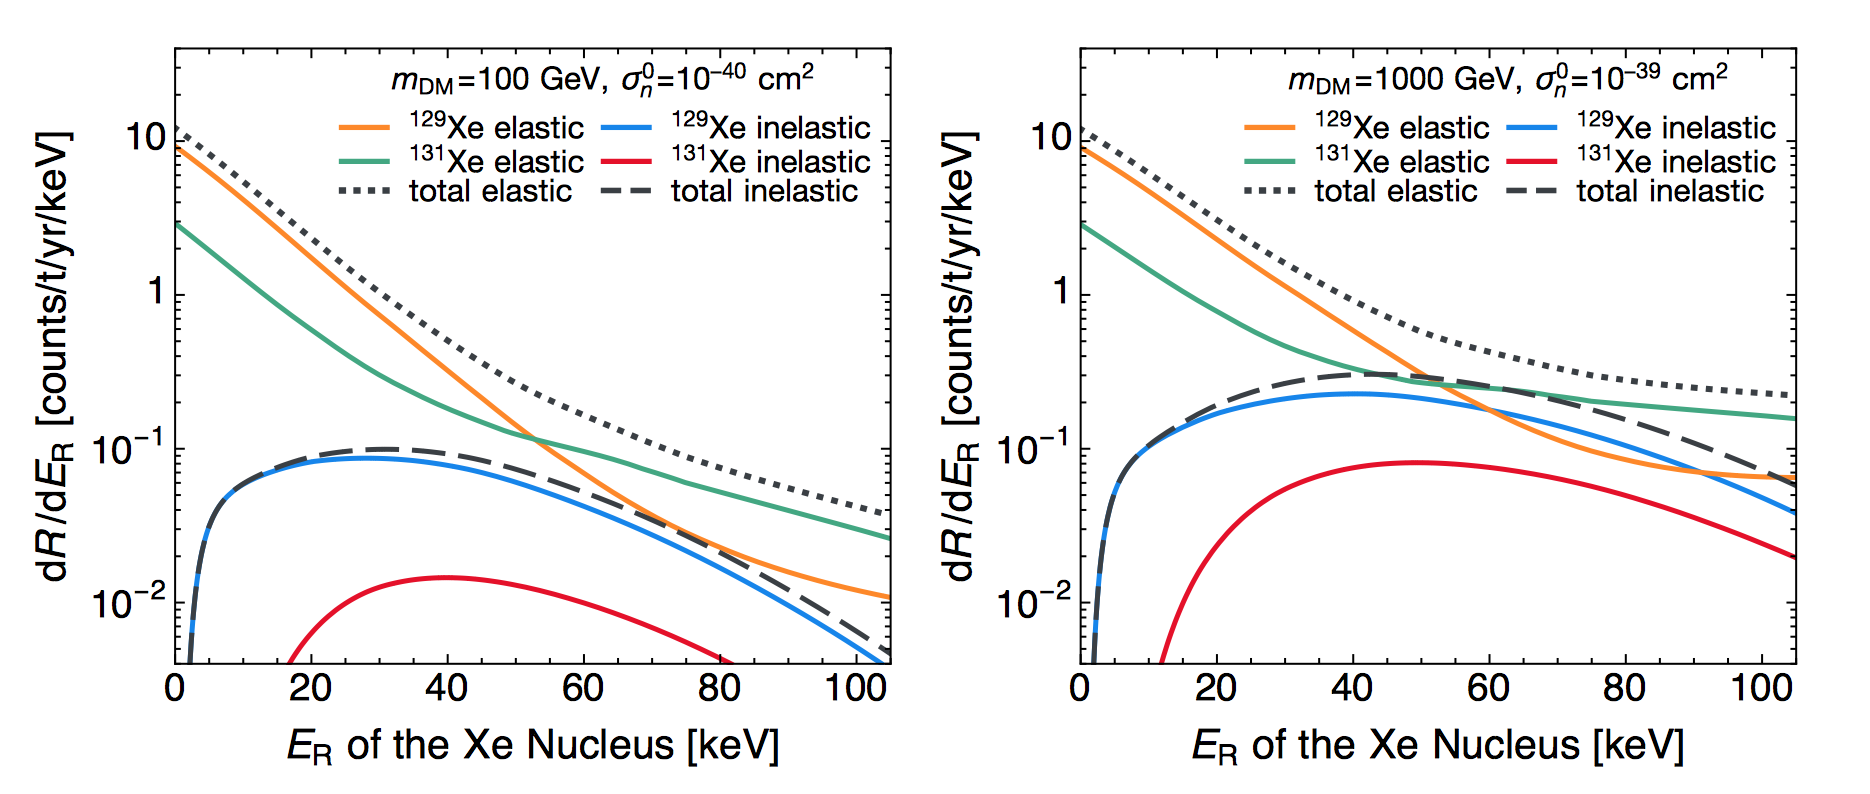
\includegraphics[width=\textwidth]{ElasticInelasticRates}
\caption{Spin-dependent recoil spectra for \ce{^{129}Xe} and \ce{^{131}Xe} for elastic and inelastic scatters.  WIMP masses
of of $100\ \mathrm{GeV/c^2}$ with cross section $\sigma_{n}^{0} = 10^{-40}\ \mathrm{cm^{2}}$
and $1000\ \mathrm{GeV/c^2}$ with cross section $\sigma_{n}^{0} = 10^{-39}\ \mathrm{cm^{2}}$ are assumed.  Elastic scattering
is preferred across all recoil energies, though at larger $E_{\mathrm{R}}$ and $m_{\chi}$ inelastic has a greater relative
impact.  Inelastic scattering drops to 0 at 
$E_{R} = 0\ \mathrm{keV}$ because conservation of momentum mandates that the nucleus cannot be excited while the atom remains at rest
after an interaction.  Image credit: \citeref{McCabe2016}.}
\label{fig:nr_elastic_inelastic}
\end{figure}

The final kind of interaction is elastic scattering and preserves kinetic energy.  Elastic scatters probe both spin-independence
and spin-dependence.  \figref{fig:nr_elastic_inelastic} shows the expected recoil spectra for \ce{^{129}Xe} and
\ce{^{131}Xe} elastic and
inelastic scatterings for WIMPs of $m_{\chi} = 100,\ 1000\ \mathrm{GeV/c^2}$ with cross-sections of
$\sigma_{n}^{0} = 10^{-40},\ 10^{-39}\ \mathrm{cm^{2}}$.  We see that elastic scattering is dominant over inelastic, but at higher recoil
energies $E_{R}$ and larger WIMP masses the gap of the discrepancy decreases.  This suggests a spin-dependent dark matter discovery should
be first observed with elastic scatters.  From here on elastic scattering will be the primary focus since it is used for the
spin-independent search (a few sections will focus on $\mathrm{^{129m}Xe}$ and $\mathrm{^{131m}Xe}$).


%====================================
\section{Electronic Recoils}
\label{sec:er}
Xenon will undergo an electronic recoil when its electron shell interacts with a moving particle.  Because no energy
is lost to atomic motion the number of quanta produced is

\begin{equation}
n_{\mathrm{q}} = \frac{E}{W}
\label{eq:nquant_er}
\end{equation}

\noindent where $W = 13.7 \pm 0.2\ \mathrm{eV}$ \citeref{Dahl2009} is the energy required to produce a single quantum.  This is made up
of

\begin{equation}
n_{\mathrm{q}} = n_{\mathrm{ex}} + n_{\mathrm{ion}}
\label{eq:quanta}
\end{equation}

\noindent where \nex and \nion is the numbers of excitons and ions, respectively.  The number of electron-ion pairs has a root mean square
of

\begin{equation}
\delta = F \times n_{\mathrm{ion}}
\label{eq:fano}
\end{equation}

\noindent where $F < 1$ is known as the Fano factor \citeref{Fano1947}.  Thus the fluctuations of $n_{\mathrm{ion}}$ are smaller than a
Poisson distribution ($F = 1$).  Several experiments have attempted to measure $F$ for LXe \citeref{Doke1976, Seguinot1995} and
estimate a value of $F = 0.059$ for \electron and $\gamma$-rays.  This places a limit on the fundamental energy resolution of

\begin{equation}
\Delta E = \sqrt{F W E}
\end{equation}

\noindent where it is common to measure $\Delta E$ is in keV, $W$ is in eV, and the energy $E$ is in MeV \citeref{Aprile2009}.  Current
LXe experiments have not yet achieved a Poisson resolution, so there is a lot of progress that can be made in the future.

Rearranging \eqnref{eq:quanta} the probability that a quanta is an ion is

\begin{equation}
p_{\mathrm{ion}} = \frac{1}{1 + \frac{ n_{\mathrm{ex}} }{ n_{\mathrm{ion}} }}
\end{equation}

\noindent with $p_{\mathrm{ex}} = 1 - p_{\mathrm{ion}}$.  The ratio $n_{\mathrm{ex}} / n_{\mathrm{ion}}$ has been calculated to be
0.06 \citeref{Takahashi1975}
but later measurements disagree \citeref{Doke2002, Aprile2007}.  Currently $n_{\mathrm{ex}} / n_{\mathrm{ion}}$ is expected to be
between 0.06-0.2.  Following recombination the number of photons and electrons is

\begin{subequations}
\begin{align}
n_{\mathrm{ph}} &= n_{\mathrm{ex}} + rn_{\mathrm{ion}} \\
n_{\mathrm{e}} &= (1 - r)n_{\mathrm{ion}}
\end{align}
\end{subequations}

\noindent where \nphot is the number of photons and \nelect is the number of \electron that do not recombine.

Although noble gas detectors allow ER-NR discrimination, the two regions are near one another some events could
be considered with reasonable probability to belong to either.  In dark matter searches only the region of NR-space where the NR
likelihood is significantly more probable is used (\secref{sec:dark_matter_results}).  A number of reduction methods are used to minimize
the electronic recoil and other backgrounds.  With the ton-scale era of DM detectors
underway this becomes especially critical, and significant effort has been put into material screening and distillation.


%====================================
\section{Nuclear Recoils}
\label{sec:nr}
Although the vast majority of background comes from electronic recoils, nuclear recoils are more dangerous because they replicate
WIMP interactions.  Therefore the NR background must be well-modeled to avoid mistaking background with WIMPs.

A fraction of the energy in a nuclear recoil will increase the kinetic energy of the xenon.  Liquid noble gas detectors cannot measure
changes in translational motion of atoms so this portion is lost.  While energetic electrons are capable of transferring very small
amounts of energy to the motion of the nucleus, the reverse is not true.  Atomic motion has only been observed in nuclear recoils,
which implies for the same energy deposition $n_{\mathrm{q}}$ will differ between electronic and nuclear recoils.  The fraction of energy
not lost to atomic motion $f_{n}$ is commonly described by the Lindhard model
\citeref{Lindhard1965}

\begin{equation}
f_{n} = \frac{k g(\epsilon)}{1 + k g(\epsilon)}
\label{eq:linhard_quenching}
\end{equation}

\noindent where $k = 0.133Z^{2/3}A^{1/2}$, $g(\epsilon) = 3\epsilon^{0.15} + 0.7\epsilon^{0.6} + \epsilon$, and
$\epsilon = 11.5 (E / Z^{7/3})$ where $Z$ is the atomic number, $A$ is the number of nucleons, and $E$ has units of keV.  $k$ is
proportional to the ratio of
electronic stopping power to particle velocity of the recoiling Xe atom \citeref{Sorensen2011} and $g(\epsilon)$ is proportional
to the ratio of electronic to nuclear stopping power (\secref{subsec:stopping_power}) \citeref{NEST2015}.  Here $k$ is taken
from \citeref{Lewin1996} but there has been some debate over its value.  When parameterized by the Lindhard model the quenching factor
$f_{n}$ is sometimes written as $L(E)$.  It is shown in \figref{fig:lindhard} for the relevant energy search region.

\begin{figure}
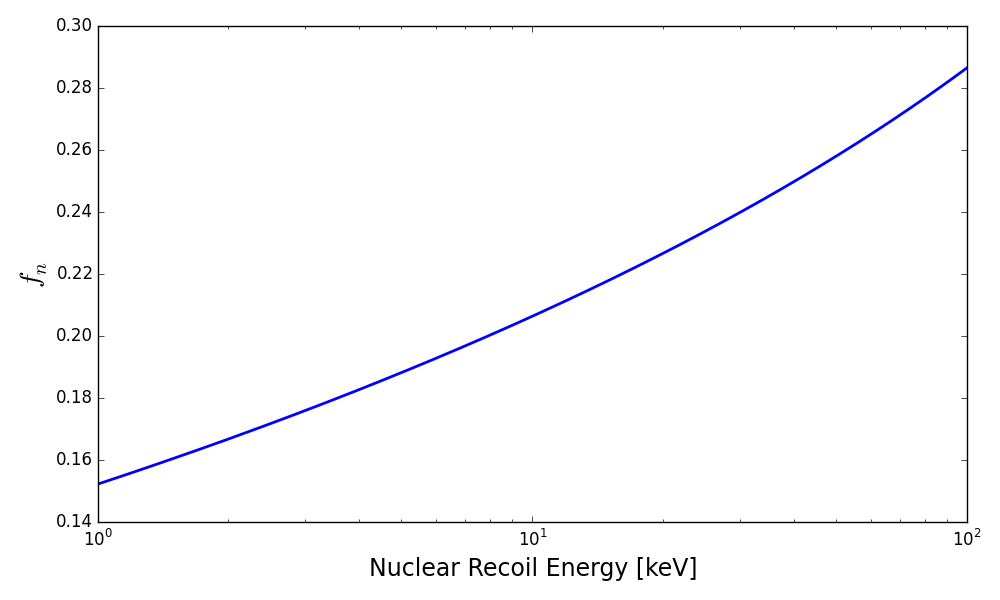
\includegraphics[width=0.8\textwidth]{Lindhard}
\caption{Fraction of nuclear recoil energy that causes excitons and ions in xenon using Lindhard's theory \citeref{Lindhard1965}.}
\label{fig:lindhard}
\end{figure}

Primary scintillation is reduced by biexcitonic quenching and the Penning process (\eqnref{eq:nr_scint_quench}).  The total
number of quanta is

\begin{equation}
n_{\mathrm{q}} = L(E) \frac{E}{W}
\label{eq:nquant_nr}
\end{equation}

\noindent The difference between \eqnref{eq:nquant_er} and \eqnref{eq:nquant_nr} is $L(E)$.  As with electronic recoils the probability
of a quantum being an ion is

\begin{equation}
p_{\mathrm{ion}} = \frac{1}{1 + \frac{ n_{\mathrm{ex}} }{ n_{\mathrm{ion}} }}
\end{equation}

\noindent through the higher track density of nuclear recoils (\figref{fig:er_nr_recoil_diagram})  causes
$n_{\mathrm{ex}} / n_{\mathrm{ion}} \sim 1$ \citeref{Sorensen2011, Angle2011}.  As electrons and ions
recombine biexcitonic quenching and the Penning process reduce the number of photons by $f_b$ (\eqnref{eq:nr_scint_quench}).

\begin{subequations}
\begin{align}
n_{\mathrm{ph}} &= f_b ( n_{\mathrm{ex}} + rn_{\mathrm{ion}} ) \\
n_{\mathrm{e}} &= (1 - r)n_{\mathrm{ion}}
\end{align}
\end{subequations}



%====================================
\section{Time Projection Chambers}
\label{sec:tpcs}
Time projection chambers (TPCs) measure the light and charge of an interaction.  They have been leading the
spin-independent search for WIMP masses $> 10\ \mathrm{GeV/c^2}$ for ${\sim}10\ \mathrm{years}$, and as we reach the ton-scale era are
projected to continue.  \figref{fig:sensitivity_evo} shows the evolution of detectors and their spin-independent limits for roughly
$30 \mdash 70\ \mathrm{GeV/c^2}$ WIMPs.  This section discusses liquid noble gas TPCs used for dark matter detection.  It primarily covers
xenon but for most details an identical treatment can be applied to argon and neon.

\begin{figure}
\centering
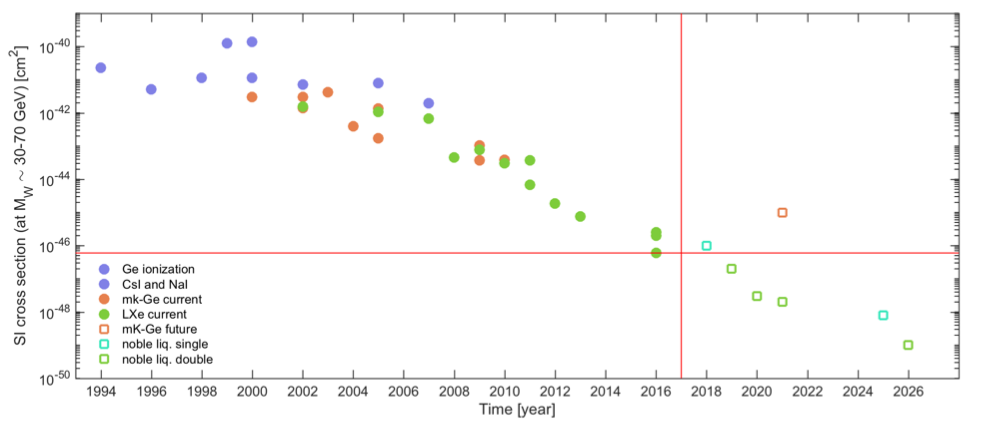
\includegraphics[width=0.9\textwidth]{SensitivityEvolutionBetter}
\caption{Spin-independent cross-section evolution for WIMPs with $m_{\chi} \sim 30 \mdash 70\ \mathrm{GeV/c^2}$.  Solid markers represent
realized
values while empty squares denote projected.  Purple markers refer to germanium (\secref{subsec:germanium}) as well as CsI and NaI
detectors (\secref{subsec:crystals}), orange represent cryogenic bolometers (\secref{subsec:bolometers}), turquoise denotes single-phase
noble liquid chambers, and green symbolizes dual-phase.  For approximately the last decade LXe detectors have led the search and are
projected to continue to do so.  Image credit: \citeref{Baudis2014}.}
% for SensitivityEvolution
%Black circles refer to germanium and silicon detectors (\secref{subsec:germanium}), blue diamonds
%depict cryogenic bolometers (\secref{subsec:bolometers}), red and green triangles symbolize LXe and LAr detectors, and
%purple squares represent bubble chambers (\secref{subsec:bubbles}).  Image credit: \citeref{Undagoitia2016}.}
\label{fig:sensitivity_evo}
\end{figure}

\subsection{Working Principle}
\label{subsec:tpcs_working_principle}
TPCs consist of a liquid noble element with a small gas gap at the top.  A minimum of three parallel metal meshes are needed: the
cathode, gate, and anode.  The cathode is
at the bottom of the detector and applies an electric field - known as the drift field $E_d$ - inside the active volume.  The gate rests
just beneath the liquid level and is grounded, so the drift field pushes electrons that do not recombine towards the surface of the liquid
at drift velocity $v_{d}$.  Typically an electric field cage consists
of metal rings that mark the perimeter and are stacked vertically, parallel to the cathode and gate.  Identical resistors connect adjacent
rings so voltage drops are equivalent and maintain drift field uniformity.

The observable that corresponds to the measurement of photons emitted from the site of the interaction is referred to as the S1, named
because it is the first scintillation.  The electrons, which do not contribute to the S1, drift to the surface of the liquid.  Over this
period the electron cloud diffuses longitudinally (in the direction of $E_{d}$) and transversely (perpendicular).  The
diffusion coefficients $D_{L}$ and $D_{T}$ are dependent on the electric field with $D_{T}/D_{L} \sim 10$.  The electron spread can
be written as $\sigma_{D_{T}} = \sqrt{D_{T} t_{d}}$ where $t_{d} = d/v_{d}$ is the electron drift time and $d$ is the drift distance.

Impurities that outgas from detector materials mix into the gas and liquid.  Electronegative impurities in particular are a problem
because they attach to drifting $e^{-}$ and
lower the number that reach the liquid-gas interface.  The attachment process
is \eqnref{eq:impurity_attach}.

\begin{equation}
e^{-} + S \rightarrow S^{-}
\label{eq:impurity_attach}
\end{equation}

\noindent where $S$ is an impurity.  The number of \electron captured depends on drift time and the impurity attachment rate
$k_{S}$, both of which vary with $E_{d}$.  An advantage of larger electric fields is a greater
\vd (up to a point, \figref{fig:drift_velocity}) to limit time in the liquid.  Doping LXe with organic materials such as butane
can increase \vd at large
fields but are not used in DM detectors because of purification difficulties \citeref{Yoshino1976}.  The rate at which electrons are
absorbed by impurities is proportional to the number of electrons, impurities, and impurity attachment rate.  Assuming the density
of impurities in the liquid and $E_{d}$ are uniform the charge $q$ is described by

\begin{equation}
\frac{dq}{dt} = -qk_{S}S
\label{eq:lifetime_diff_eq}
\end{equation}

\begin{equation}
q(t) = q_{0}e^{-tk_{S}S} = q_{0}e^{-t/\tau_{e}}
\label{eq:lifetime_equation}
\end{equation}

\noindent where $\tau_{e} = (k_{S}S)^{-1}$ is the electron lifetime and $q_0$ is the initial charge.  $k_{S}$ is the attaching rate
constant and is shown in \figref{fig:attachment_rate} for O$_{2}$,
N$_{2}$O, and SF$_{6}$.  It increases for N$_{2}$O with $E_d$ whereas \otwo and SF$_{6}$
decerase.  For LXe TPCs it is common to give the impurity concentration in \ce{O_2}-equivalence - the concentration of \otwo if it were
solely responsible for \electron attachment.  \ce{O_2} is expected to be the dominant electronegative contaminant, and its curve
in \figref{fig:attachment_rate} works well for modeling the electron lifetime (\chapref{chap:purification}).  Removing these
impurities is discussed in \secref{subsec:xenon1t_pur} and measuring the electron lifetime is covered in
\secref{subsec:det_char_elifetime, sec:electron_lifetime_measurements}.

\begin{figure}
\includegraphics[width=0.8\textwidth]{attachingratevsfield}
\caption{Attaching rate constant $k_{S}$ for O$_{2}$, N$_{2}$O, and SF$_{6}$ with respect to electric field.  At
larger $E_d$ $k_{S}$ increases for N$_{2}$O and decreases for \otwo and SF$_{6}$.  Image credit: \citeref{Bakale1976}.}
\label{fig:attachment_rate}
\end{figure}

The anode rests several millimeters above the gate.  The electric field between the gate and anode $E_{g}$ must be strong
enough to extract the \electron that reach the liquid surface into the gas (typically $\gtrsim 10\ \mathrm{kV\ cm^{-1}}$).  An extracted
\electron will quickly gain enough kinetic energy to ionize atoms in the gas,
whose \electron in turn follow, creating a cascade effect.  Because the scintillation per electron is independent of
the total number of electrons extracted this is known as proportional scintillation.  It is also known as secondary scintillation or
electroluminescence.  The number of photons $N_{\mathrm{ph}}$ produced over a distance $z$ per electron is

\begin{equation}
\frac{dN_{\mathrm{ph}}}{dz} = \alpha \bigg( \frac{E_{g}}{P} - \beta \bigg) P
\label{eq:electronlum}
\end{equation}

\noindent where $\alpha = 70\ \mathrm{photons\ kV^{-1}}$, $\beta = 1.0\ \mathrm{kV\ cm^{-1}\ atm^{-1}}$, and $P$ is the pressure in the
gas \citeref{Belogurov1995}.  The observable that corresponds to the measurement of electroluminescence is referred to as the S2, for
second scintillation.


\subsection{Photomultiplier Tubes}
\label{subsec:tpcs_pmts}
Photomultiplier tubes (PMTs) are used for light detection in TPCs.  A digram of a PMT is shown in \figref{fig:tpcs_pmts_pmt_diagram}.  A
photon that
passes through the PMT window will most often strike the photocathode and free a photoelectron via the photoelectric effect.  This process
is known as single photoelectron emission (SPE).  Once ejected, the photoelectron will be directed by the focusing electrode towards the
first dynode.  The dynodes are coupled to one another through resistors that systematically decrease their electric potential.  As the
photoelectron hits the first dynode it will free a second electron.  The freed electrons will be drawn to the
second dynode and repeat this procedure.  The result is a cascade effect, amplifying the current by as much as 100 million and ending
at the anode, where the charge is output to a voltage reading device such as an oscilloscope or digitizer.

\begin{figure}
\centering
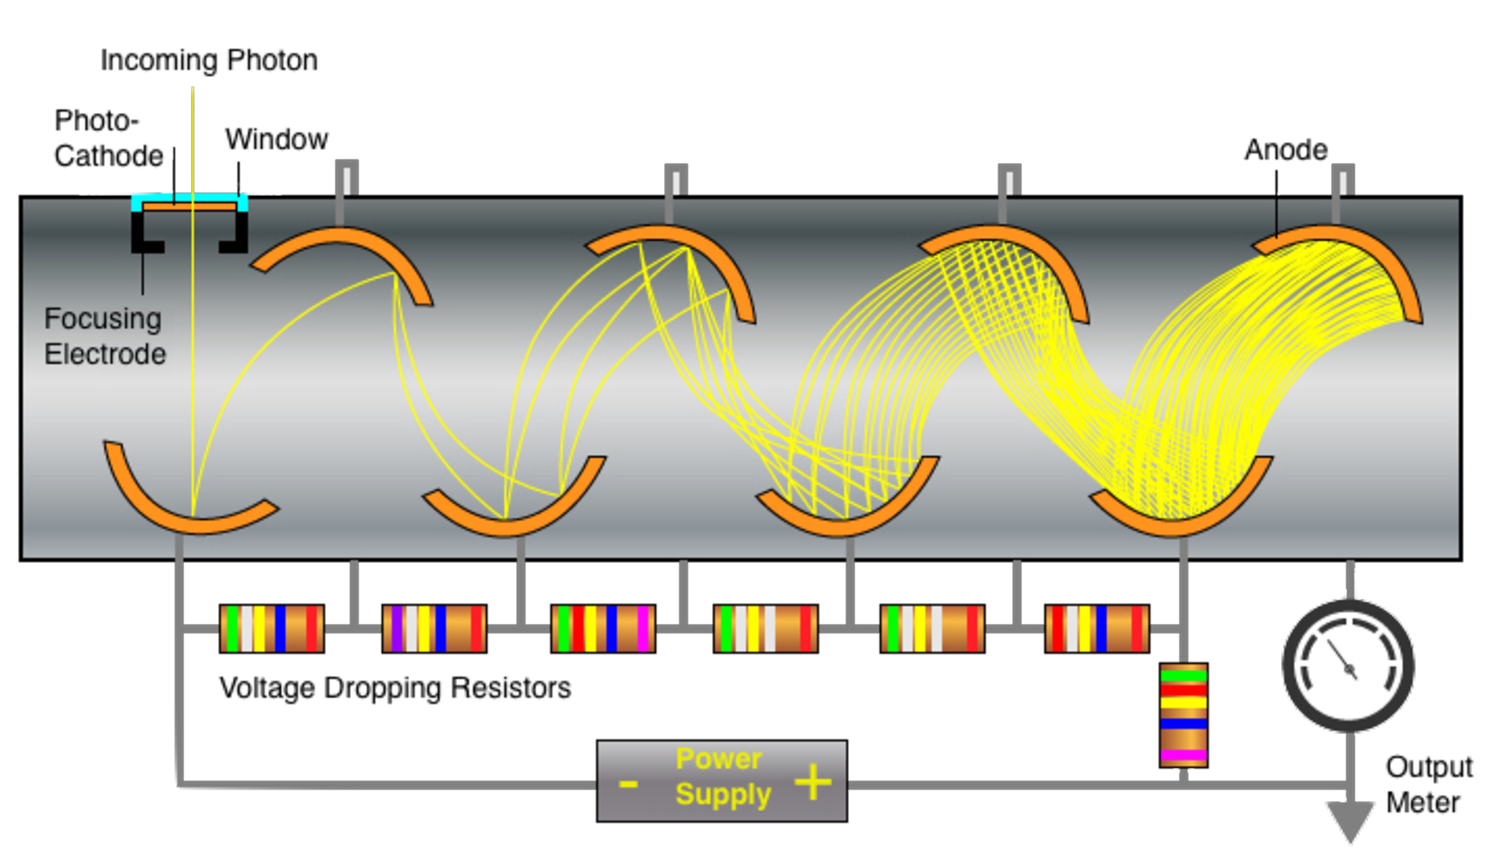
\includegraphics[width=0.8\textwidth]{PMT1Better}
\caption{Diagram of a PMT.  An incident photon hits the photocathode and ejects an photoelectron.  With each dynode the more \electron are
freed, creating an amplified signal.  Image credit: \citeref{CHROMacademy}.}
\label{fig:tpcs_pmts_pmt_diagram}
\end{figure}

If the photon's energy is at least double the workfunction of the photocathode the number of photoelectrons ejected should follow
follow a Poisson distribution.  However, a study of several Hamamatsu vacuum ultraviolet-sensitive (VUV) PMTs showed double
photoelectron emission
(DPE) fractions between 18-24\% depending on the PMT, higher than the expected ${\sim} 15\%$ \citeref{Faham2015}.  The study included PMTs
used in XENON100 and XENON1T.  In other cases a photon may pass through the photocathode and hit
the first dynode.  If it ejects an electron the PMT response
will be similar to a photocathode hit with one less dynode, i.e. an under-amplified current.  

The quantum efficiency (QE) is the ratio of electrons ejected from the photocathode divided by incident photons.  The QE spectrum for
the PMTs used in XENON1T, Hamamatsu R11410, is shown in \figref{fig:tpcs_pmts_qe}.  Its low efficiency means the majority of photons that
reach our PMTs will not produce a photoelectron.  Other photodetectors have been considered but lead to problems that outweigh those
of PMTs.  Xenon's scintillation wavelength (178 nm) is near the spectrum's maximum of approximately 35\%.  Liquid argon and neon have
scintillation wavelengths of 128 and 78 nm, respectively.  Because PMTs are not sensitive to these energies LAr experiments use
wavelength shifters.

\begin{figure}
\centering
\includegraphics[width=0.6\textwidth]{pmt_efficiency}
\caption{Quantum efficiency with respect to wavelength for the Hamamatsu R11410 PMT, used in XENON1T.  The peak efficiency occurs near
the xenon scintillation wavelength 178 nm at ${\sim} 35 \%$.  Image credit: \citeref{Lung2012}.}
\label{fig:tpcs_pmts_qe}
\end{figure}

TPCs have photomultiplier tubes below the cathode and above the gate.  While proportional scintillation occurs at the top of the detector
and in most detector settings produces enough light to guarantee detection, prompt scintillation - especially for low energy events - can
be more difficult to observe.  Depending on the geometry of the detector and the location of the event the fraction of light
directed towards the photodetectors can
be small.  PMTs cannot be fixed around the side of the TPC because their electric fields will interfere with the field
cage.  To increase
the fraction of light that reaches the photodetectors the wall of the TPC is covered by polytetrafluoroethylene (PTFE) just inside the
field cage.  PTFE is reflective for liquid noble gas scintillation and is a common choice.  It has been shown to have $> 97 \%$
reflectance to 178 nm light when immersed in LXe \citeref{Neves2017}.



\subsection{Signals}
\label{subsec:tpcs_signals}
S1s (primary scintillation) and S2s (secondary) are measured in photoelectrons (PEs).  An example of an
event is shown in \figref{fig:tpcs_signal_tpc}.  On the left a particle scatters with the LXe, prompting photons that are almost
immediately observed by the PMTs.  The right side shows the \electron drifting to the LXe surface and
extracted by the anode across the GXe.  The colors correspond to the relative intensity of light seen by each PMT.  For a typical S1 the
bottom PMTs observe more light due to reflection off the LXe surface (though the amount depends on where in the TPC the interaction
occurs).  For S2s the top PMTs see more light since electroluminescence occurs just several centimeters underneath them.  For S2s
the top PMTs have an intensity profile centered around where the \electron are extracted.  The profile for the bottom PMTs is more
uniform since the solid angle per PMT is less.

\begin{figure}
\centering
\includegraphics[width=\textwidth]{xenon1t_tpc}
\caption{Diagram of an interaction in a LXe TPC.  The S1 is immediately
observed by the PMTs.  The \electron drift towards the top of the detector, where they are extracted across GXe,
creating the S2.  A typical waveform is shown at the bottom.  The S2 is significantly
larger than the S1 due to the amplification of electroluminescence.  The relative intensity of light in the PMTs, or PMT hit
pattern, can be used to determine the $x$- and $y$-coordinates of the interaction.  Image credit: Lutz Alth\"{u}ser.}
\label{fig:tpcs_signal_tpc}
\end{figure}



\subsubsection{Position Reconstruction}
\label{subsubsec:tpcs_signals_posrec}
In addition to knowing the $z$-coordinate of the interaction ($z = v_{d} t_{d}$) TPCs can recover the $x$ and $y$ positions.  The S2
hit pattern in the top PMT array in \figref{fig:tpcs_signal_tpc} shows an intensity distribution that peaks at one
PMT and dissipates away from it.  It is reasonable to assume the S2 was extracted beneath or nearly beneath this PMT.  A number of
algorithms can be applied to PMT hit patterns to estimate the $x \mdash y$ position of the event.  Typically the resolution of event
reconstruction depends on the number and area of PMTs as well as the S2 size.  \figref{fig:tpcs_signals_posrec} shows the event
distribution for second XENON1T science run.  The majority of events are near the wall - a consequence of
radioactivity present in detector materials.  The large self-shielding of LXe constrains these events to ${\sim}5\ \mathrm{cm}$ of the
wall.  Three-dimensional position reconstruction allows us to reject events in regions where we
expect a large background.  The region of interest for dark matter search data is known as the fiducial volume.

\begin{figure}
    \centering
    \begin{subfigure}[t]{0.45\textwidth}
        \centering
        \includegraphics[height=4.5cm]{PosRecXY}
    \end{subfigure}%
    \begin{subfigure}[t]{0.45\textwidth}
        \centering
        \includegraphics[height=4.5cm]{PosRecRZ}
    \end{subfigure}
    \caption{Position reconstruction for events in XENON1T Science Run 1.  Top PMT hit patterns are used to determine $x \mdash y$ while
    $z = v_{d} t_{d}$.  The number of events drops dramatically at lower radii due to the self-shielding of LXe.}
	\label{fig:tpcs_signals_posrec}
\end{figure}



\subsubsection{Discrimination}
\label{subsubsec:tpcs_signals_discr}
The exciton-to-ion ratio and recombination (\secref{subsec:recombination}) are responsible for the fraction of quanta that produce S1s
and S2s.  Under identical
detector conditions recombination is largely governed by the ionization density, which is determined by the stopping power
(\secref{subsec:stopping_power}).  \figref{fig:mass_stopping_power} shows the mass stopping power dependence on energy and recoil type,
and \figref{fig:er_nr_recoil_diagram} shows the track structure for 20 keV electronic and nuclear recoils.  Because the nuclear recoil has
a greater ionization density its electron-ion pairs are more likely to recombine \citeref{Faham2014}.  The disproportionate exciton-to-ion
ratios and recombination fraction allow discrimination between electronic and nuclear recoils.

\figref{fig:tpcs_signals_ernr} shows S2 vs. S1 for electronic and nuclear recoils.  The ER are from \ce{^{220}Rn} calibrations
where its progeny \ce{^{212}Pb} undergoes $\beta$-decay.  The short lifetime of the \ce{^{220}Rn} decay chain, continuous energy spectrum
of $\beta$-decays, and uniform distribution throughout the detector make \ce{^{220}Rn} an excellent choice for measuring S1 and S2 for
electronic recoils.

To map the S1-S2 parameter spaces separate ER and NR calibrations are performed.  Electron recoil calibrations use \ce{^{220}Rn} since
its progeny \ce{^{212}Pb} undergoes $\beta$-decay.  The short lifetime of the \ce{^{220}Rn} decay chain
($\sum_i t_{1/2} < 12\ \mathrm{h}$), continuous energy spectrum
of $\beta$-decays, and uniform distribution throughout the detector make it an excellent choice for measuring S1 and S2 for
electronic recoils.  Events from XENON1T calibrations are shown in red in \figref{fig:tpcs_signals_ernr}.

There are no neutron sources that can be mixed with xenon to perform internal nuclear recoil calibrations.  Therefore, calibrations
must be done with sources placed outside of the detector.  Xenon's self-shielding (${\sim}10\ \mathrm{rm}$ mean free path for MeV
neutrons \citeref{Israelashvili2015}) causes the distribution of events to be largest near
the source, and - depending on the size of the detector - can significantly reduce the fraction of events that reach the center of the
detector, and force longer calibration windows.  For XENON1T nuclear recoil sources include
americium beryllium \ce{^{241}AmBe} and a deuterium-deuterium (D-D) neutron generator (NG) \citeref{Lang2018}.  The nuclear recoils are
marked in blue in \figref{fig:tpcs_signals_ernr} are from the \ambe calibration during the second XENON1T science run.

As predicted above \figref{fig:tpcs_signals_ernr} shows nuclear recoils have a larger photon-to-electron ratio than electronic recoils due
to their higher $n_{\mathrm{ex}}/n_{\mathrm{ion}}$ and recombination.  It shows

\begin{equation}
\bigg( \frac{\mathrm{S}2}{\mathrm{S}1} \bigg)_{\mathrm{ER}} > \bigg( \frac{\mathrm{S}2}{\mathrm{S}1} \bigg)_{\mathrm{NR}}
\end{equation}

\noindent across all S1-S2 values.  This data is used to characterize the ER and NR observables (S1, S2) space so that the origin of each
dark
matter search event can be estimated.  Because a substantial fraction of energy is lost to atomic motion in a nuclear recoil the energies
of the events in \figref{fig:tpcs_signals_ernr} differ between ER and NR.  As an example, a nuclear recoil event at
$\mathrm{S1} = 60\ \mathrm{PE}$ has an energy of ${\sim}35\ \mathrm{keV}$ while for electronic recoils it is closer to 8 keV.  For this
reason several energy scales are used (\secref{subsubsec:tpcs_signals_energy}).

\begin{figure}
\centering
\includegraphics[width=\textwidth]{er_nr_discrimination}
\caption{S2 (proportional) vs. S1 (prompt) for XENON1T calibration data.  Electronic recoils are from the \ce{^{220}Rn} decay chain as
progeny \ce{^{212}Pb} undergoes $\beta$-decay with an end-point energy of 569.9 keV (red).  Nuclear
recoils are from americium beryllium (\ce{^{241}AmBe}) (blue).  S2/S1 is larger for electronic recoils, which enables discrimination
between possible WIMPs and the ER background.}
\label{fig:tpcs_signals_ernr}
\end{figure}

The number of photons and electrons can be reconstructed from the S1 and S2.  Doing so requires knowledge of a number of detector
variables including PMT quantum efficiencies (\secref{subsec:tpcs_pmts}) and electroluminescence
(\secref{subsec:tpcs_working_principle}).  These are discussed in detail in \secref{sec:det_char} and
\secref{sec:er_nr_calibrations_parameter_determ}.  If the energy of an event is known the light yield and charge yield can be calculated
in units of photons per energy and electrons per energy, i.e. $n_{\mathrm{phot}}/E$ and $n_{\mathrm{e}}/E$.  Because the light and charge
yields describe detector-independent microphysics there has been an effort to measure them
(\secref{sec:er_nr_calibrations_results_ly_qy}).  Measurements of photoelectrons per energy may also be referred to as light and charge
yields (\secref{subsec:det_char_ly_cy}) and are useful for monitoring detector conditions (because they are detector-dependent they do not
provide insight into fundamental physics).  \figref{fig:tpcs_signals_drift_field} shows the ratios of light and
charge yields as a function of drift field for 122 keV electronic recoils (\ce{^{57}Co} $\gamma$-rays), 56.5 keV elastic nuclear recoils
(\ce{^{241}AmBe} and \ce{^{252Cf}}), and
5.3 MeV $\alpha$-decays (\ce{^{210}Po}).  At larger $E_d$ the light yield declines while the charge yield increases.  The more
significant change in ER is due to its sparser ionization density and suggests the drift field can be optimized for ER-NR discrimination.

\begin{figure}
\centering
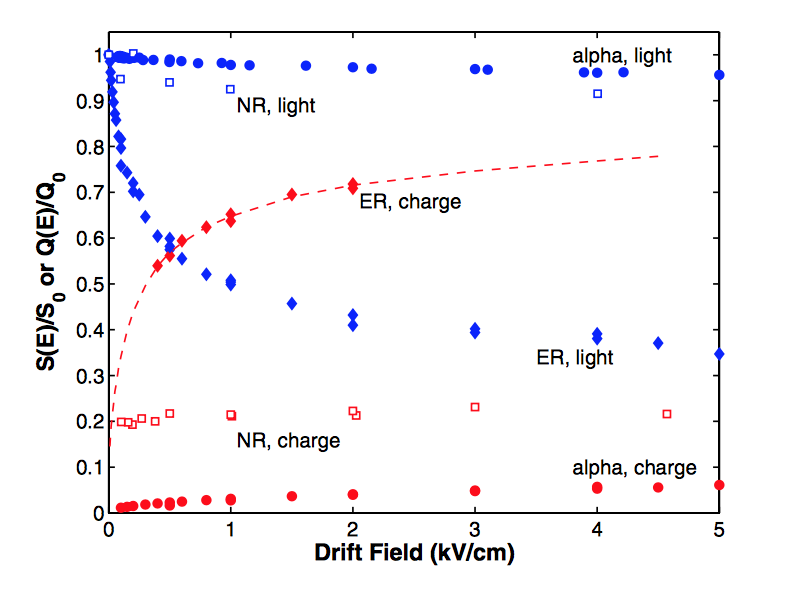
\includegraphics[width=0.8\textwidth]{LYQY}
\caption{Field dependence of light (S(E)/S$_{0}$, red) and charge (Q(E)/Q$_{0}$, blue) yields.  S$_{0}$ is the light yield at zero field
and Q$_{0}$ is the charge yield at
infinite field.  Electronic recoils are shown as solid diamonds and are measured from \ce{^{57}Co} 122 keV $\gamma$-rays.  56.5
keV elastic neutron scatters from \ambe and \ce{^{252}Cf} are marked by hollow squares.Nuclear recoils
are marked by hollow squares and are from elastic 56.5 keV neutron scatters from \ambe and \ce{^{252}Cf}.  Solid circles represent \ce{^{210}Po}
5.3 MeV $\alpha$-decays.  Sparser ionization densities precipitate stronger field-dependence for electronic scatters than for nuclear and
alpha, signifying $E_{d}$ can be tuned for improved ER-NR discrimination.  Image credit: \citeref{Aprile2006b}.}
\label{fig:tpcs_signals_drift_field}
\end{figure}



\subsubsection{Energy Reconstruction}
\label{subsubsec:tpcs_signals_energy}
An important feature in a detector is the ability reconstruct the energy of the event.  There are several energy scales used
depending on the interest.  For electronic recoils energy
reconstruction is relatively straightforward since the energy is converted to photons and electrons.  Nuclear recoils are more
complicated since they pick up translational energy and are more likely to undergo biexcitonic quenching.  There are three commonly-used
energy scales.

The \textbf{electronic recoil equivalent energy} is the name for conversion between \gammaray and detector response of scintillation or
ionization, generally measured in PE.  It can be used to identify mono-energetic $\gamma$ lines, which are useful im defining the energy
scale.  If only the S1 or S2 is measured the energy is typically specified since the recombination fraction varies with energy.  The units
are given as ``$\mathrm{keV_{ee}}$'' for electron-equivalent.

The \textbf{electron equivalent combined energy scale (CES)} uses the primary and proportional scintillations to reconstruct $E$.  This is
only used for electronic recoils since, unlike nuclear recoils, energy is not lost to xenon nuclei (either as kinetic energy or nuclear
excitation).  Using this scale we can reconstruct our background energy spectrum (ERs are $> 99\%$ of total background).

The ``electron-recoil equivalent energy" scale is used for the conversion of signal to energy using $\gamma$-rays.  It uses either the S1 or
S2 and has units of photoelectrons or electrons, respectively.  It has units of $\mathrm{keV_{ee}}$ for ``electron-equivalent".  Because
recombination varies with respect to energy this scale will be non-linear, so it is common to include the energy used in the
calibration.

``Nuclear-recoil equivalent energy" is based on nuclear recoil primary scintillation.  For historical reasons it is defined using the
122 keV \gammaray from \ce{^{57}Co}.  It is given by

\begin{equation}
E_{\mathrm{NR}} = \frac{S1 S_{\mathrm{ER}}(E)}{L_{y,\mathrm{ER}} \mathcal{L}_{eff} S_{\mathrm{NR}}(E)}
\end{equation}

\noindent where $L_{y,\mathrm{ER}}$ is the electronic recoil light yield at 122 keV, $\mathcal{L}_{eff}$ is the relative nuclear
recoil
scintillation efficiency, and $S_{\mathrm{ER,NR}}(E)$ are the scintillation quenching factors for ER and NR, respectively.  Units are
given in \kevnr for ``nuclear-equivalent".

The ``combined energy scale" uses both S1 and S2.  This is beneficial because natural fluctuations between photons and electrons at a
given energy are now accounted for (\eqnref{eq:nphot_ne}).  In addition it typically leads to better energy resolution because both signals
are used, and recombination variation over energy does not lead to non-linearity.  Typically several $\gamma$ sources are used to
construct it, so it takes units of $\mathrm{keV_{ee}}$.






















% for stopping power look at A Model of Nuclear Recoil Scintillation Efficiency in Noble Liquids
%D.-M. Mei a,∗ Z.-B. Yin a,b,1, L.C. Stonehill c, A. Hime c


%Lewin and Smith (1996) - Lindhard factor
%Doke et al., 2002 - LET
%Miller et al., 1968 - drift velocity








% for kr/xe level
%E Aprile, J Aalbers, F Agostini, M Alfonsi, F. Amaro, M Anthony, F Arneodo, P Barrow, L Baudis, B. Bauermeister, et al., “Removing krypton from xenon by cryogenic distillation to the ppq level,” The European Physical Journal C, vol. 77, no. 5, p. 275, 2017.